%   Filename    : chapter_3.tex 
\chapter{Research Methodology}
\label{sec:methodology}

This chapter discusses the materials and methods to be employed in the study, focusing on the development requirements and the software and languages utilized. This will also entail the overall workflow in conducting the study, Non-Invasive Methods in Determining the Sex of \textit{Tegillarca granosa} (blood cockles) using machine learning technologies. The different machine/deep learning algorithms will be thoroughly discussed to ensure a comprehensive understanding of the entity of the research endeavor and its processes. 

Dr. Victor Emmanuel Ferriols, the director of the Institute of Aquaculture, will oversee the overall workflow and conduct of this experiment. The researchers will also be guided by the research associates, LC Mae Gasit and Allena Esther Artera. Consequently, the whole dataset collection process will be done at the University of the Philippines Visayas hatchery facility. 



\section{Sample Collection}
\label{sec:samplecollect}
A total of 500 adult \textit{T. granosa} that have already spawned will be used in this experiment wherein their sex was already classified as male or female. The sample sizes are going to range from 34 to 61 mm and will be sourced from the coastal area in the municipality of Zaraga, Iloilo, Philippines, as well as from fish markets in the municipality of Ivisan, Capiz, Philippines. The research and experimentation will be done at the University of the Philippines Visayas hatchery facility in Miagao, Iloilo, Philippines. The samples will be placed in 200 L fiberglass reinforced plastic (FRP) tanks containing filtered seawater with 35 ppt salinity \cite{miranda2023} and will be subjected to spawning to categorize male from female \textit{T. granosa}. The samples will undergo a series of temperature fluctuations to induce the spawning of gametes as described in the study of Ferriols and Miranda (2023). This method, induced spawning, is the most natural and least invasive method for bivalves compared to other methods \cite{aji}. Thus, after the spawning, there would be 500 classified males and 500 classified females. 

\begin{figure}[!htbp]
	\centering
	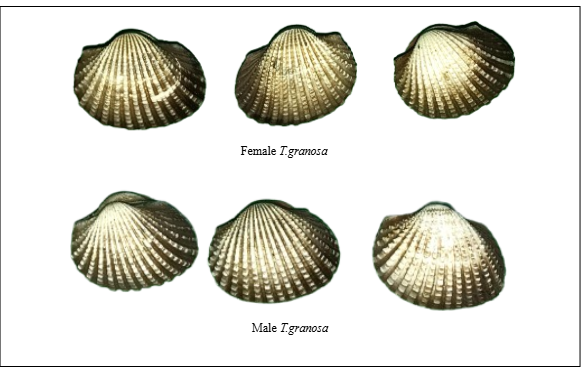
\includegraphics[width=0.9\textwidth]{figures/male-female T.granosa.png}
	\caption{Male and Female \Tegillarcagranosa shell.}
\end{figure}

\section{Ethical Considerations}
\label{sec:ethical}

Ethical approval was not required for this study involving animals, as per local legislation and institutional guidelines, because the experiments were conducted only on species that are commonly used as food and intended for human consumption. 


\section{Creating \textit{T. granosa} Dataset}
\label{sec:dataset}

For the initial preparation of the experiment, the researchers will collect primary observations for 100 samples of \textit{T. granosa.} For the actual experimentation, the researchers will collect the original dataset by batch eventually comprising 500 samples of \textit{T. granosa}. The images captured for the dataset will be saved in png format with a file naming convention of the sample’s sex, the orientation or view of the shell, and its corresponding number out of the total 1000 samples. Female \textit{T. granosa} samples will begin with 0 in their file name, while males will begin with 1, followed by the views captured such as (1) dorsal, (2) ventral, (3) anterior, (4) posterior, (5) left lateral, and (6) right lateral, and lastly, a unique sample number. For example, “010001” will be the file name for the first female sample taken from the dorsal view and “110001” for the first male sample also taken from the dorsal view. The dataset will be organized in a CSV file that lists each image’s file name along with their shell’s width, height, length, rib count, length of the hinge line, and distance between their umbos. This dataset will be essential for machine learning model training and testing. 

\section{Morphological Characteristics Collection}
\label{sec:morphochar}

Morphology refers to the biological form and represents one of the most visually recognizable phenotypes across all organisms \cite{tsutsumi2023}. Morphology is a term that describes structural characteristics by measuring specific components, namely, dimensions such as shapes, sizes, and colors. As stated by the researchers, quantifying and characterizing the shape is essential to understanding and visualizing the variations in \textit{T. granosa’s} morphology. 
In this study, the researchers are going to measure the height, width, and length of \textit{T. granosa.} The dimensions will be recorded using a Vernier caliper to the nearest 0.01 mm. The length of the \textit{T. granosa} refers to the measurement from the anterior to the posterior of the shell, the width will be measured through the shell’s widest point from the left to the right valve and lastly, the height will be measured from the base of the shell to the shell’s apex. The height of the gap between the valves near the hinge will also be measured. The authors Reyment and Kennedy (1998), indicated that the use of counts of the shell ribs as supplementary information increases identification accuracy. Thus, the researchers will also take into account the difference in the rib count of the male and female \textit{T. granosa} and the ratio will be calculated since the sizes of the blood clams may vary.
Sex ratio, size frequency distribution, and relative growth rates were used to investigate sexual dimorphism.

\begin{figure}
	\centering
	\begin{minipage}[b]{0.24\textwidth}
		\centering
		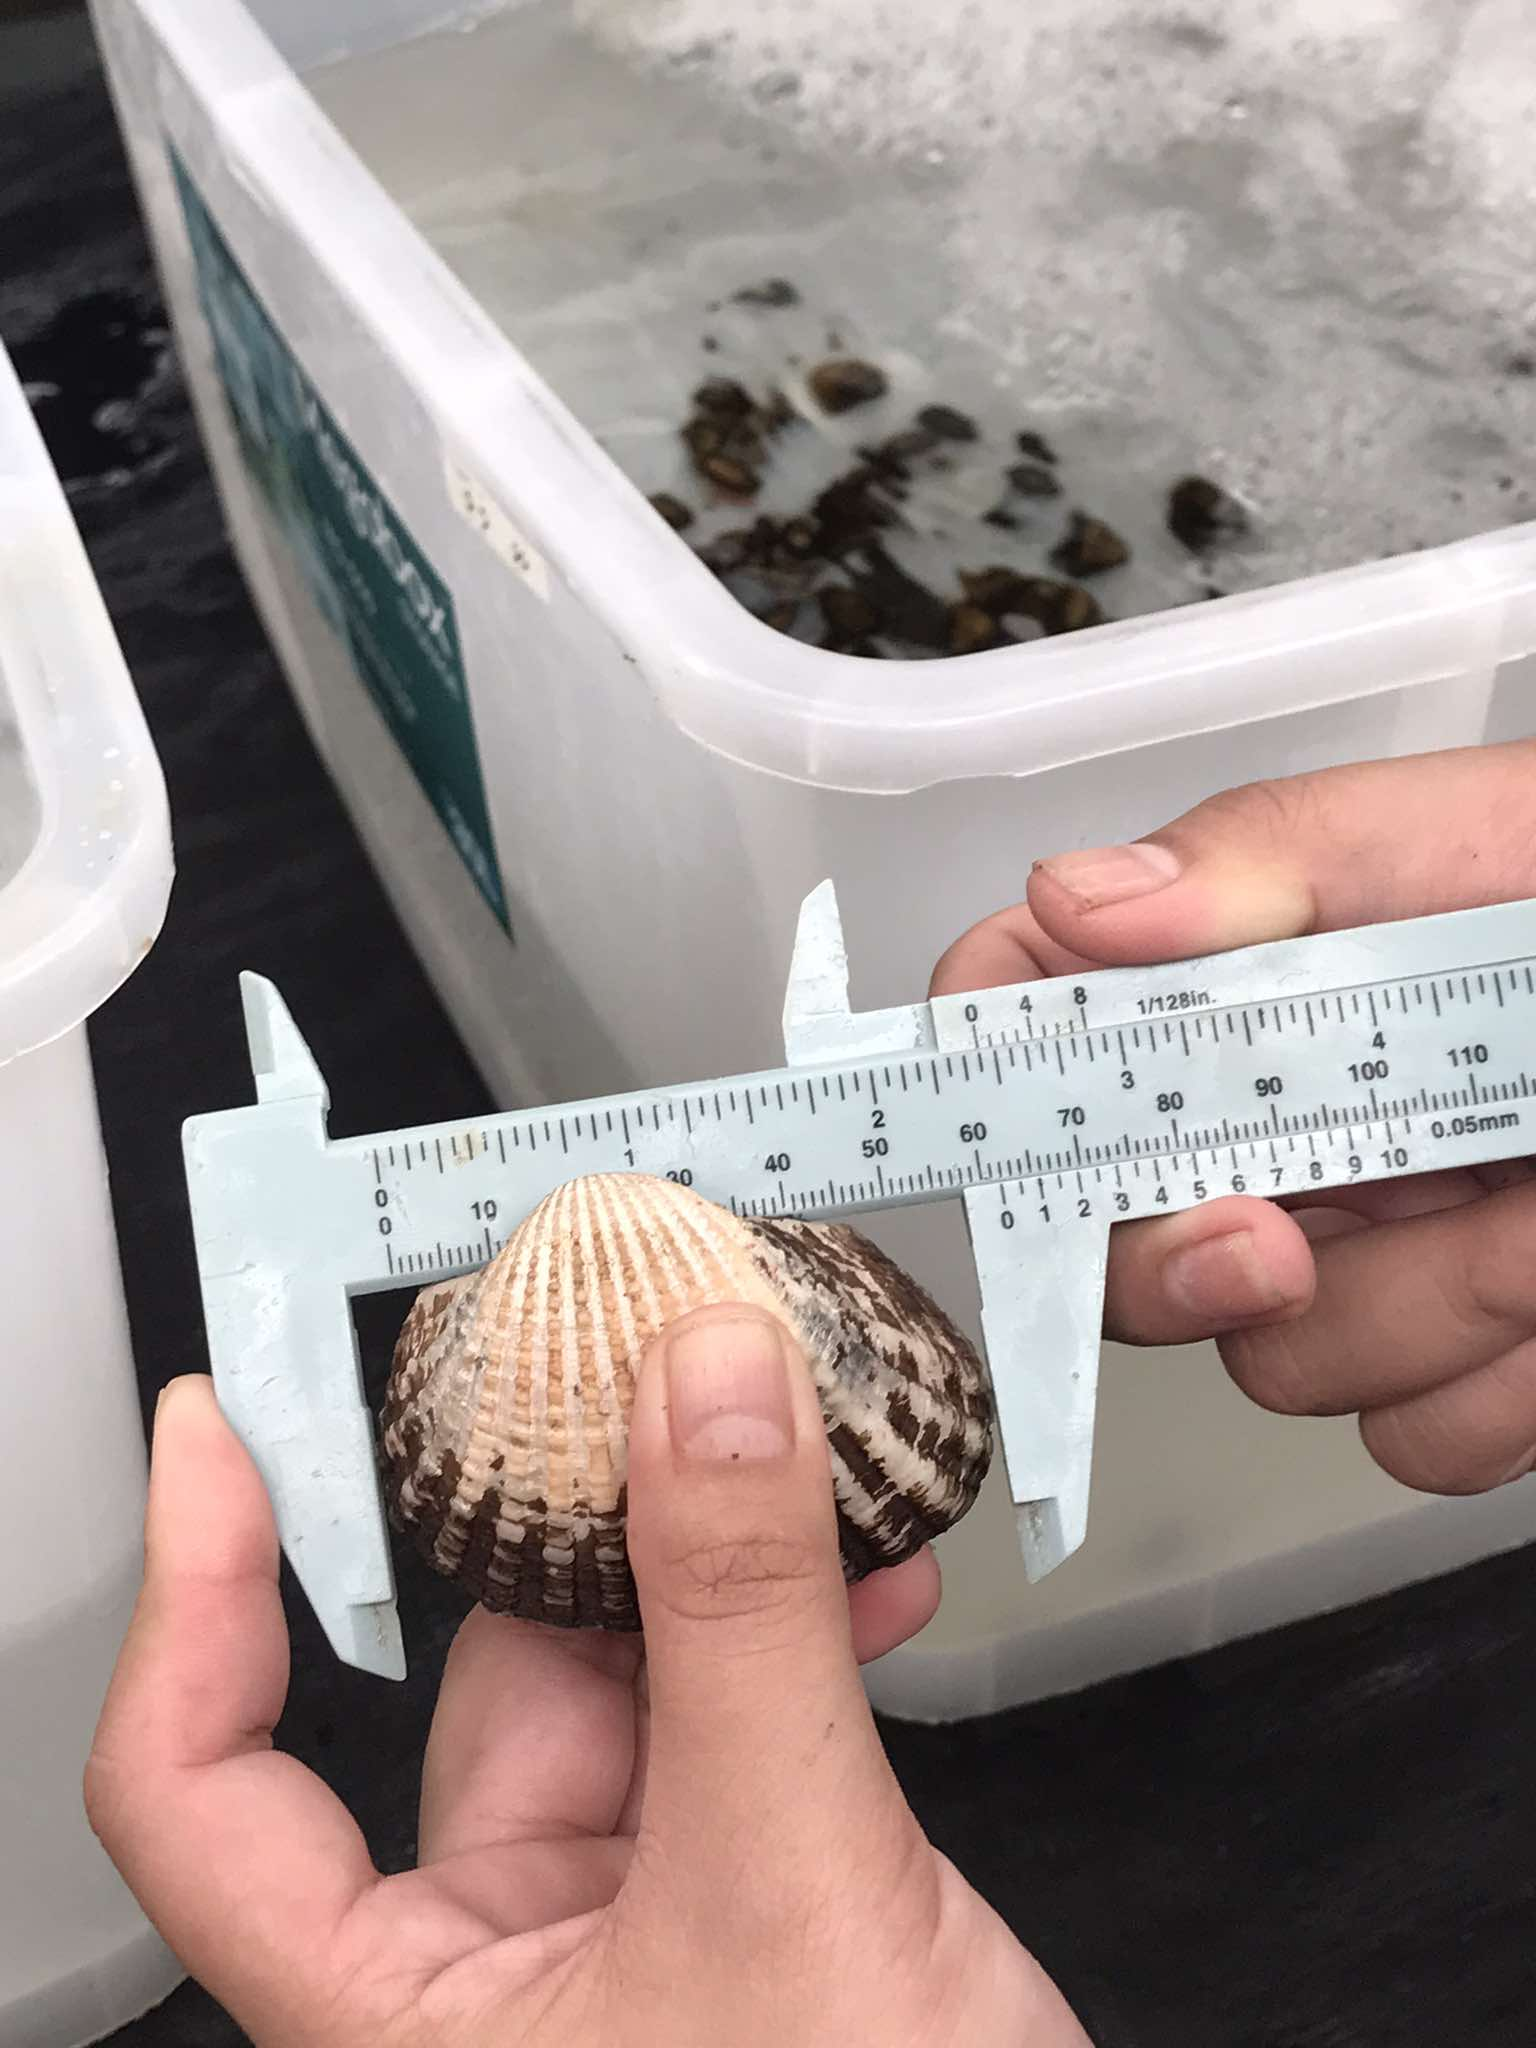
\includegraphics[width=\linewidth]{length}
		\caption{Length}
	\end{minipage}\hspace{0.4cm}
	\begin{minipage}[b]{0.24\textwidth}
		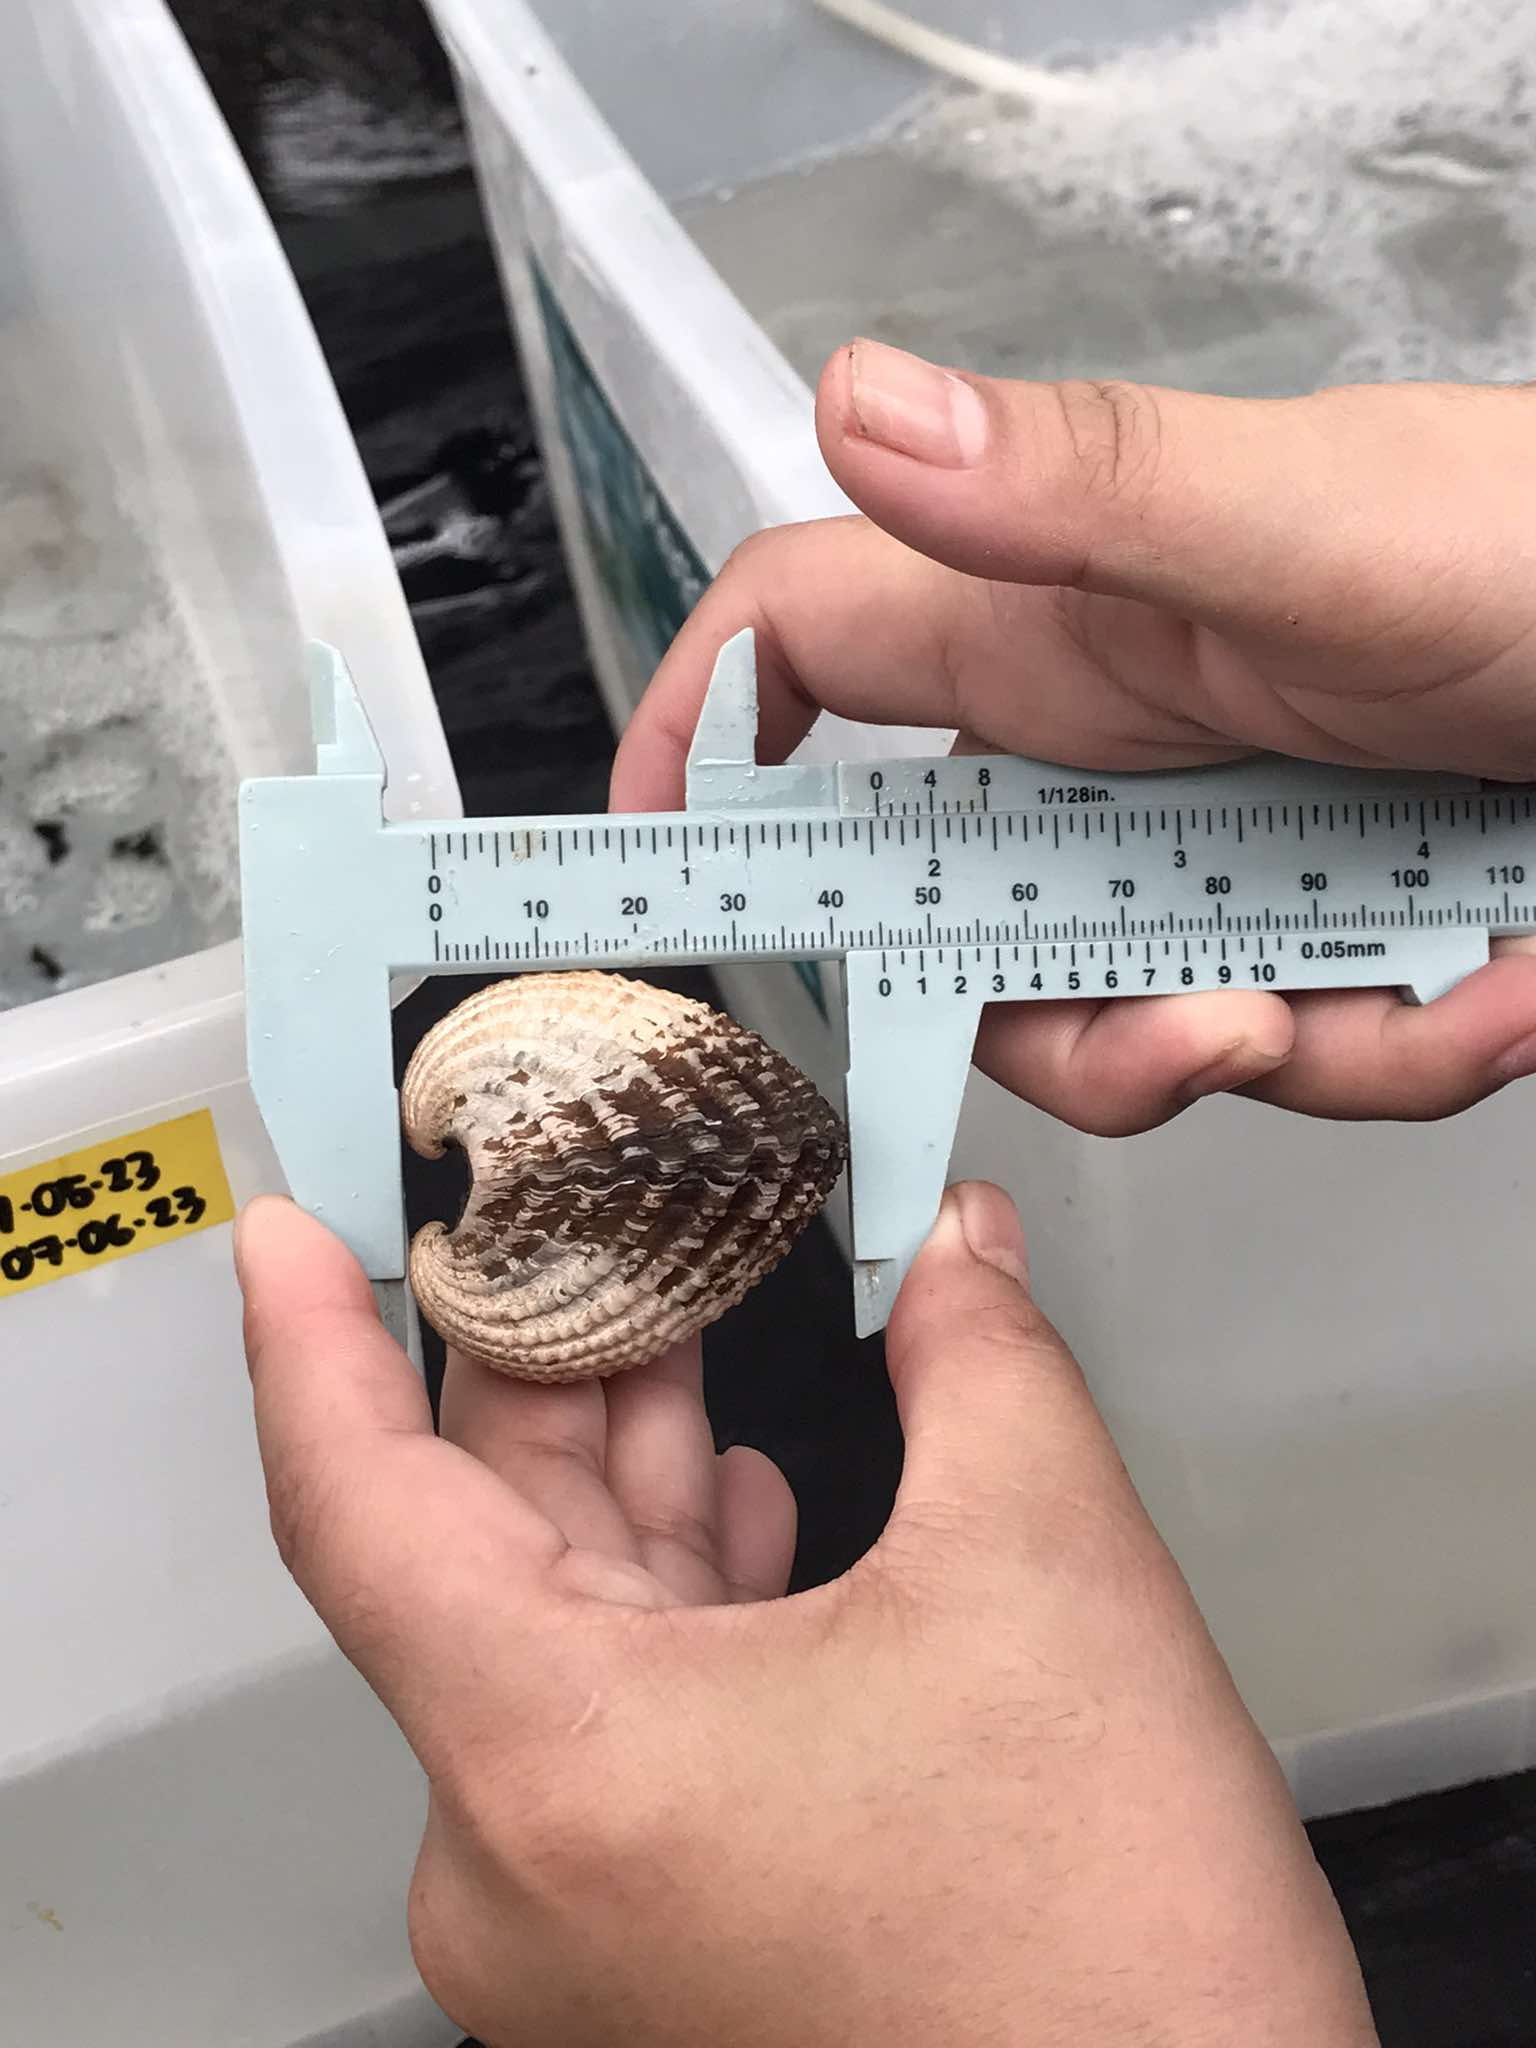
\includegraphics[width=\linewidth]{width}
		\caption{Width}
	\end{minipage}\hspace{0.4cm}
	\begin{minipage}[b]{0.24\textwidth}
		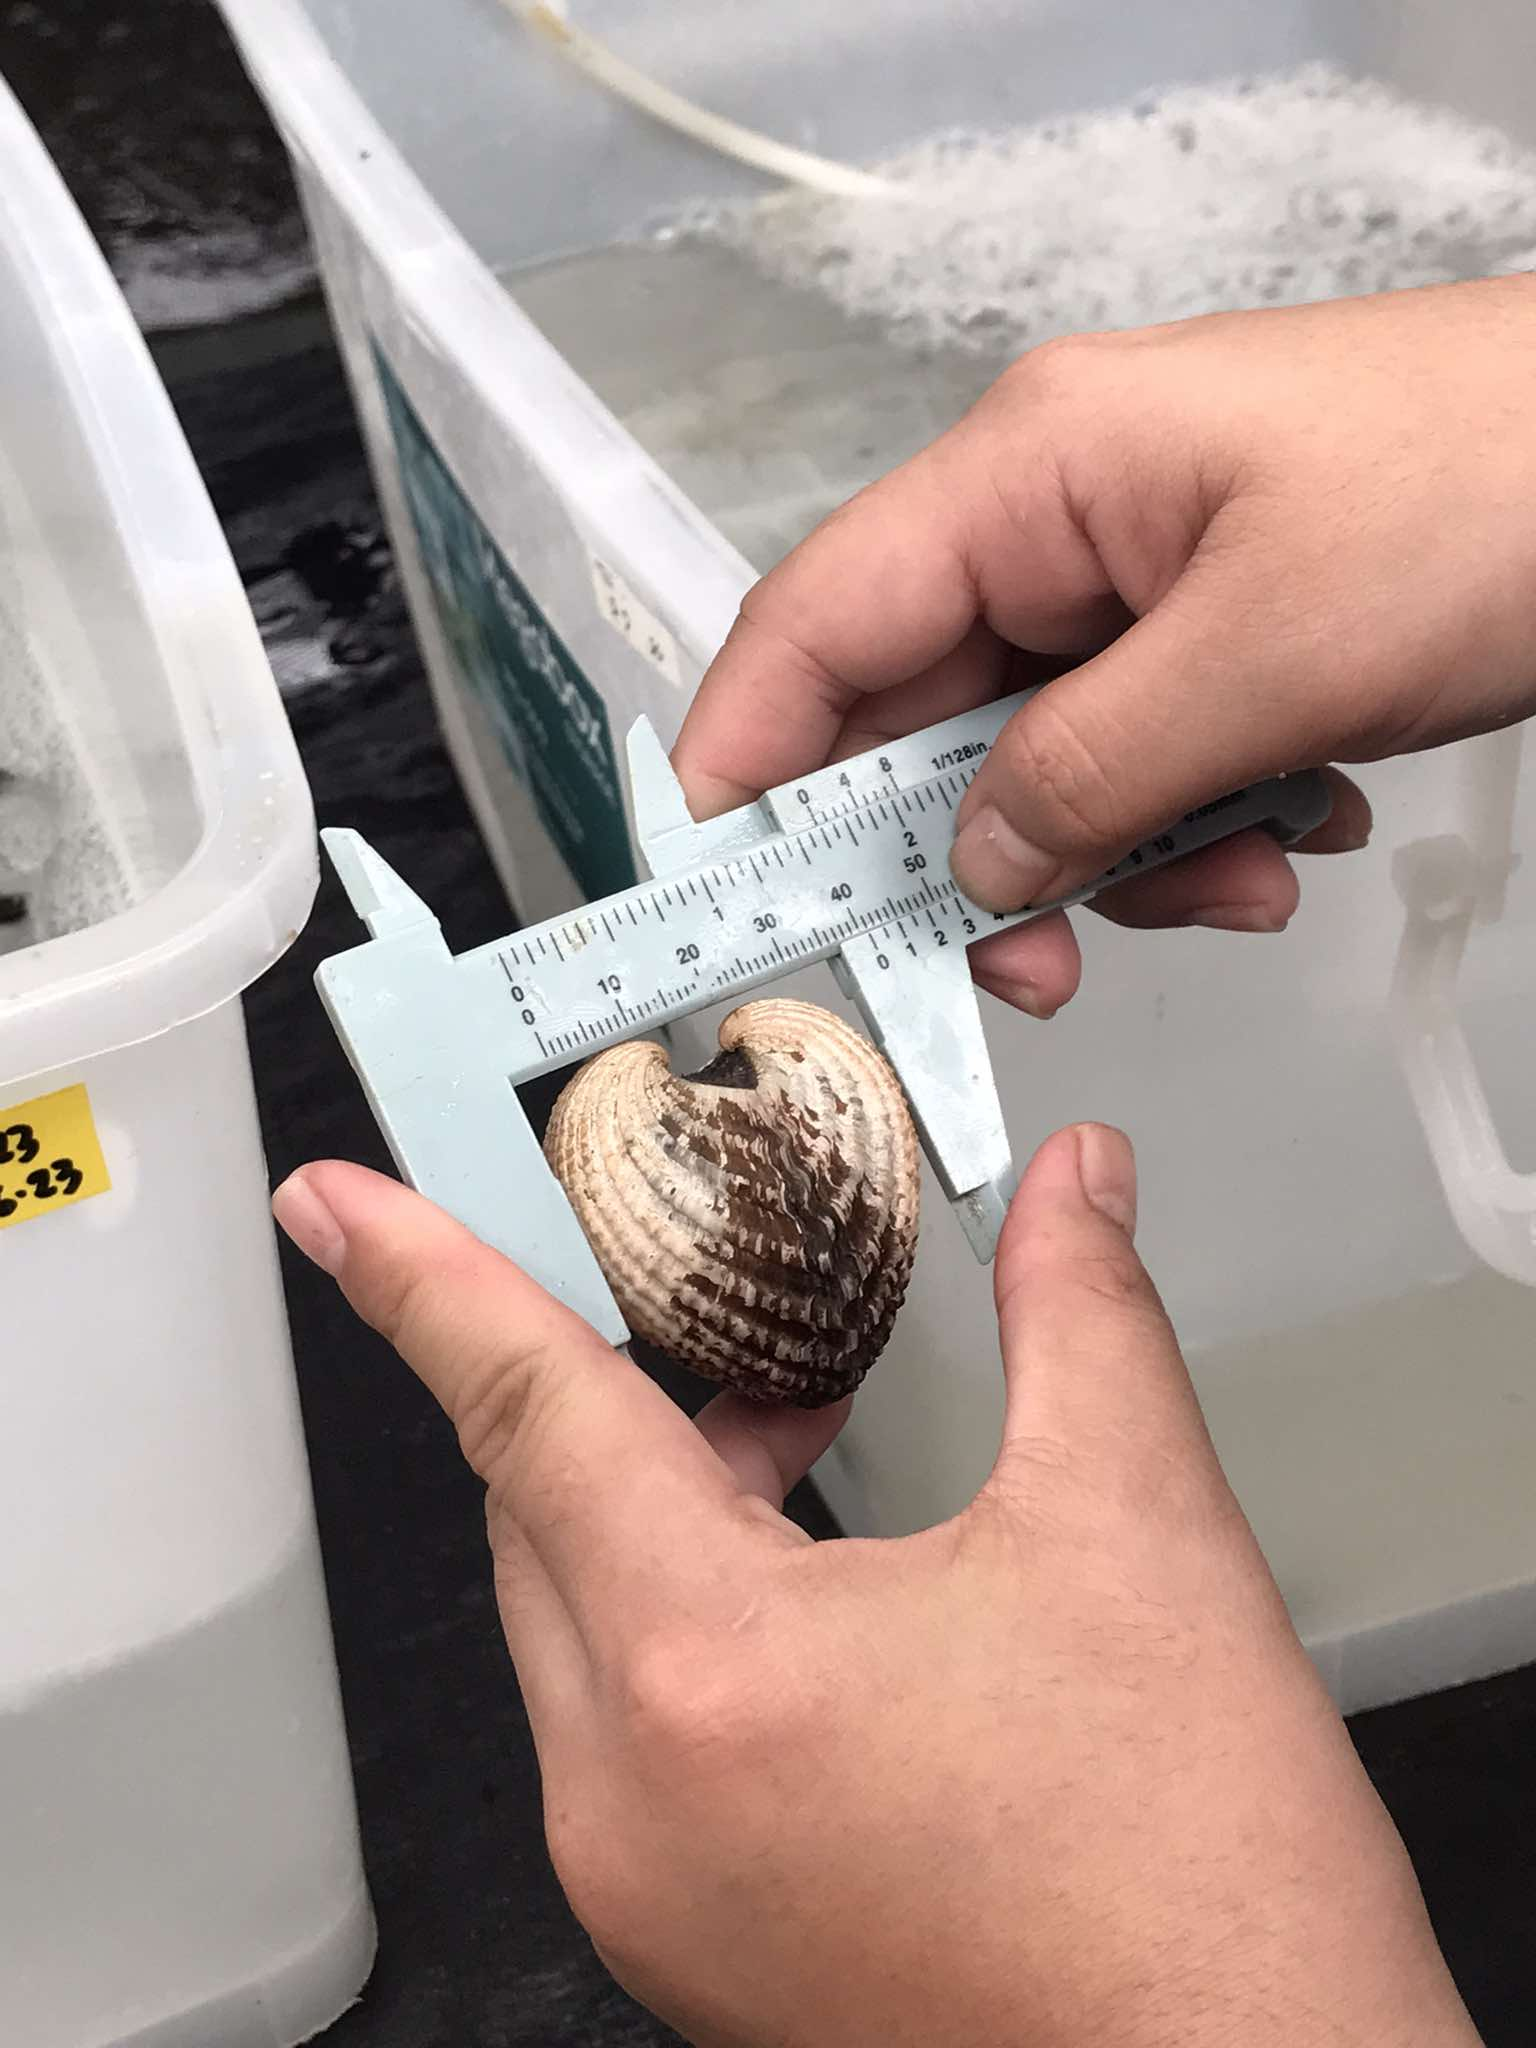
\includegraphics[width=\linewidth]{height}
		\caption{Height}
	\end{minipage}
	\caption{\textit{T. granosa’s} measurements}\label{fig:tegillarca}
\end{figure}

\section{Image Acquisition and Pre-Processing}
\label{sec:imageprocess}
In this study, there would be three major phases for the image processing to be employed namely (1) color thresholding, (2) segmentation, and (3) image hole filling and dilating. Unbalanced samples will lead to train model slowly and affect the gradient update. So, the dataset need to meet sample equilibrium criteria \cite{cui2020}. The researchers constructed a controlled environment for capturing the samples utilizing a box-like structure with a white background surface. This setup was designed to maintain uniform captures of the images, and a consistent measurement between the sample and the camera, fixing the camera at a consistent angle above the \textit{T. granosa}. Placing a ring light to the left of the box, and using a camera with flash to ensure the image quality, eliminate shadows and clarity of the sample during the image acquisition process. 

\subsection{Color thresholding}
For color thresholding, the researchers utilized the red, green, blue (RGB), hue saturation value (HSV), luminance, blue chromaticity, red chromaticity (YCbCr), and (Luminance, a, b)** (CIElab) images obtained from the smartphone considering their wide availability across various stages in the bivalve industry using the MATLAB Colour Thresholding Toolbox in determining which among the four-color spectra may generate the cleanest version of the training images with absence of any blobs . Google Pixel 3 XL will be utilized with the following specifications: 2960 x 1440 for the resolution, 4,032 x 3,024 pixels (12.2 MP) for the dimensions, f/1.8 for the fstop, 28mm (wide), ½.55”, 1.4µm, dual pixel PDAF, OIS \cite{concepcion2023}. 

\subsection{Image segmentation}
After thresholding, the lazy snapping technique will be implemented by manually drawing the background and the foreground lines that represent the black pixels and the bivalve pixels. The lazy snapping algorithm will be configured using the 20 000 superpixels which can divide the \textit{T. granosa’s} images into 20, 000 irregularly shaped geometric pixels that will be based on the CIElab gradients through K-means clustering with K = 3.

\subsection{Image hole filling and dilating}
For the last step, the researchers will perform image hole filling and dilating to ensure that no blobs are remaining that can contribute to noise which can affect the correctness of the extracted feature by taking into consideration the 200-pixel blobs that are disconnected from the largest object in its binary form. This will result in black pixels made by binary filling and dilating to remove the blobs \cite{concepcion2023}.
Image processing will be performed on the MATLAB. The images was saved on a jpg format but these images will be cropped and resized to a 64 x 64 matrix and the background of each images would be removed using the split-and-merge algorithm \cite{cui2020}. 
To ensure consistent comparisons for the analysis, the images were captured in different angles including dorsal, ventral, lateral, and anterior and posterior taken in uniform angles to provide visual coverage of the \textit{T. granosa} sample. 

\section{Hardware and Software Configuration}
The machine learning and deep learning algorithms would be trained on ACER Aspire 3 general processing unit (GPU) which has a central processing unit (CPU) of  AMD Ryzen 3 7320U with Radeon Graphics (8) @ 2.395GHz and with a memory of 8 gigabyte (GB). The model will be performed on Keras which is a deep learning framework integrated with TensorFlow \cite{cui2020}.

\section{Data Augmentation}
In the practice of deep learning, there is a possiblity of a small dataset to be filled with bias. Then the most obvious solution is to add more samples. In dealing with an unbalanced dataset which includes different data augmentation such as by means of rotating, scaling, shearing, and translating \cite{cui2020}.

\section{Machine/ Deep Learning Technologies}
This section of the paper will discuss the technologies to be used in training, and testing the model as well as associated techniques and algorithms.  Since obtaining the induced samples was done per batch, the researchers will conduct an initial run with a support vector machine before delving into more complex methods such as deep learning models. 

\section{Machine Learning Models for Pre-evaluation }
\label{sec:ml models}

The shape of recording structures was first analyzed by collecting measurements of linear distances and applying multivariate statistical methods to these data (traditional linear measurement method) \cite{rohlf1984}. Geometric morphometric (GM) methods are an alternative way of analyzing and quantifying shape, which in theory retains more detail about the geometry of the structure than could be obtained from linear measurements \cite{adams2004}. Machine learning techniques such as decision tree classification, support vector machines (SVMs), and artificial neural networks (ANNs) have been applied to the analysis of bivalve shell geometry and morphology to classify shells based on morphological features, including shell shape, size, and texture, among others \cite{kiel2021}. The results of these studies have shown that machine learning algorithms can accurately classify bivalve shells and provide insights into the relationships between shell morphology and various environmental factors.
Following this, the researchers are going to conduct a pre-evaluation of the linear measurements for 100 samples of \textit{T. granosa} using a Support Vector Machine in order to quantify whether the linear measurements can be a determining factor in determining the sex of the samples before proceeding to more complex methods. 

\subsection{Extreme Gradient Boosting}
Extreme Gradient Boosting (XGBoost) is a DT-based ensemble machine learning algorithm that combines the gradient boosting framework and decision trees to reach final decision. It has the ability to achieve improved performance and higher accuracy compared to other supervised machine learning models . This model would be beneficial in terms of its key capabilities of computation of the importance of the attributes based on the overall contribution to the accuracy of the predictions \cite{torres2023}. 

\subsection{Logistic Regression}

Logistic Regresion (LR) is the process of modeling the probability of a discrete outcome given the input variable. The outcomes in the logistic regression is measured using a binary variable and is a transformation of the linear regression using the sigmoid function \cite{cui2020}. Although, there are no related studies about sex identification in mollusks, logistic regression is useful analysis method in classification problems such as determining the sexual dimorphism given the linear measurements measured. 

\subsection{Random Forest}

Random Forest (RF) is type of supervised machine learning algorithm that is oftenly used in regression and classification problems \cite{cui2020}. It has also been utilized in mollusks studies such as sex identification of abalone wherein the Random Forest achieved the highest avaerage balance accuracy for all the datasets\cite{arifin2021}.

\subsection{Support Vector Machine}

Support Vector Machine (SVM) is a supervised machine learning algorithm that classifies data by finding the optimal hyperplane which is also used in classification and regression problems \cite{cui2020}. Support vector machine is also widely used in aquaculture related studies such as the sex determining mandible shapes of due to its ability to solve classification problems with high validation accuracy especially when the clusters of the data with varying labels. The SVM has the ability to reflect the degree of cluster separation . It has the ability to be used as tool in the variety of the image data with biological shapes \cite{tsutsumi2023}.



\section{ Deep Learning for Image-Based Classification}
\label{sec:deeplearning}
After collecting a sufficient number of images and identifying initial patterns, convolutional neural networks (CNNs) will be used. CNNs, models like VGGNet, ResNet, and Inception have been effectively applied in phenotype classification \cite{kim2024}. In this study, the deep learning model will be specifically adapted for the sex identification of \textit{T. granosa} based on shell images. CNNs will analyze the images and learn important details about their shapes that can help identify whether they are male or female. 
Unlike the approach of using three models taken by Kim et al. (2024), the researchers will focus on just one model that has shown the best performance in their study which is SqueezeNet. SqueezeNet is particularly advantageous because it reduces the number of parameters and amount of memory required to store the model without sacrificing accuracy \cite{koonce2021}. Its ability to achieve high accuracy in classifying shell images makes it a suitable choice for distinguishing between male and female \textit{T. granosa.}
Python and Keras libraries will be used to train and test the model. The dataset will be divided into training (), validation (), and testing. Performance metrics such as accuracy, precision, recall, and F1-score will be used to evaluate the model's effectiveness.
